\documentclass{article}
\usepackage[utf8]{inputenc}
\usepackage{amsmath,amsthm,latexsym,paralist}
\usepackage{courier}

\usepackage{listings}
\usepackage{color}
\usepackage{tikz}

\definecolor{dkgreen}{rgb}{0,0.6,0}
\definecolor{gray}{rgb}{0.5,0.5,0.5}
\definecolor{mauve}{rgb}{0.58,0,0.82}

\lstset{frame=tb,
  language=python,
  aboveskip=3mm,
  belowskip=3mm,
  showstringspaces=false,
  columns=flexible,
  basicstyle={\small\ttfamily},
  numbers=none,
  numberstyle=\tiny\color{gray},
  keywordstyle=\color{blue},
  commentstyle=\color{dkgreen},
  stringstyle=\color{mauve},
  breaklines=true,
  breakatwhitespace=true
  tabsize=3
}

\title{CSCE 625 Programming Assignment 3 Report}
\author{Peihong Guo~(UIN~421003404)}
\date{\today}

\begin{document}

\paragraph{Honor Code}On my honor, as an Aggie, I have neither given nor received any unauthorized aid on any portion of the academic work included in this assignment.

\paragraph{Usage} To run the program in prolog, please follow the instructions below:
\begin{enumerate}
\item Switch to correct directory: \texttt{working_directory(CWD, \textit{source_directory}).}
\item Load the program: \texttt{['path.pl'].}
\item Load the graph: \texttt{['graph.pl'].}
\item Perform query: \texttt{path(k, p, P).} or \texttt{path(a, e, P).}
\end{enumerate}

Example:
\begin{figure}[htbp]
\center
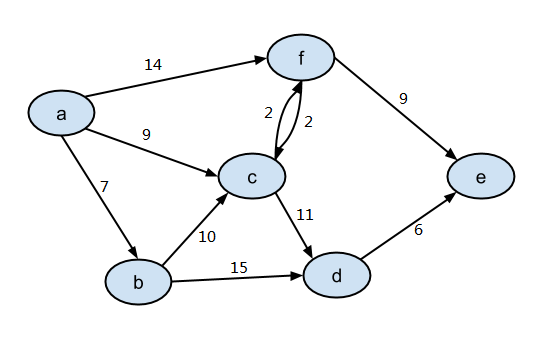
\includegraphics[width=0.6\textwidth]{./graph.png}
\end{figure}


\paragraph{Resources}

\maketitle


\end{document} 